\chapter{A GNN approach to the problem}
\label{chap:gnn}
So far we have experimented with various models trying to predict the Fock matrix as a whole. However, as has been seen in \autoref{chap:fock_matrix_predictions} this approach, which works on minimal basis sets, is not feasible for larger basis sets such as the 6-31G(2df,p) basis set. Recent advances using regression models have largely focused on separate models for each molecular species, which limits their applicability to constitutional isomers we are interested in. \parencite{ref:Hazra2024,ref:Shao2023}
We shall investigate the applicability of Graph Neural Networks (GNNs) to the problem of predicting the Fock or the density matrix. They have shown promising results in the field of quantum chemistry, especially for predicting molecular properties and structures. \parencite{ref:schnet2018}\\

The implementation of the GNN in this chapter is based on the \textsc{pytorch-geometric} framework \parencite{ref:PyTorchGeometric, ref:PyTorch_geom_paper}. 
\section{Input \& Output Matrices}
\label{sec:gnn_input_output_matrices}
Generally the input and the output of neural networks is fixed. We thus need to find a specific way to embed our input (overlap matrix) and output (Fock or density matrix) into a fixed structure. Given the nature of our problem, we can simply split our matrix representation into blocks representing the different atom sorts and their respective combinations. This yields three different types of matrix-blocks: 
\begin{itemize}
    \item \textbf{Self-blocks:} These blocks mix orbitals of the same atom type, e.g. $\text{\ch{O}}_0$ or $\text{\ch{H}}_1$\footnote{Subindices only enumerate elements and are not part of the chemical formula}. The self-blocks are diagonal blocks of the input and output matrices.
    \item \textbf{Homo-blocks:} These blocks mix only orbitals of the same atom type, e.g. $\text{\ch{H}}_1 - \text{\ch{H}}_2$.
    \item \textbf{Hetero-blocks:} These blocks mix orbitals of different atom sorts, e.g. $\text{\ch{O}}_0 - \text{\ch{H}}_2$.
\end{itemize}
Subsequently, we shall label self-blocks as node-blocks and homo- / hetero-blocks as interaction blocks interchangeably. 

A schematic depiction for the \ch{H2O} molecule using the 6-31G(2df,p) Basis is given in \autoref{fig:schematic_gnn_blocks}. Due to the symmetry of our input and output matrices we are only concerned with the upper triangular matrices for self-blocks and the homo- / hetero-blocks in the upper triangular part with respect to the full matrix. For the given example we thus have 351 entries for \ch{O} and 15 for \ch{H} self-blocks. Additionally, the \ch{H} homo-blocks yield 25 entries each and we obtain 130 values per \ch{O}-\ch{H} hetero-block. In total 666 entries suffice to reconstruct the full $36 \times 36$ matrix. 
\begin{figure}[H]
    \centering
    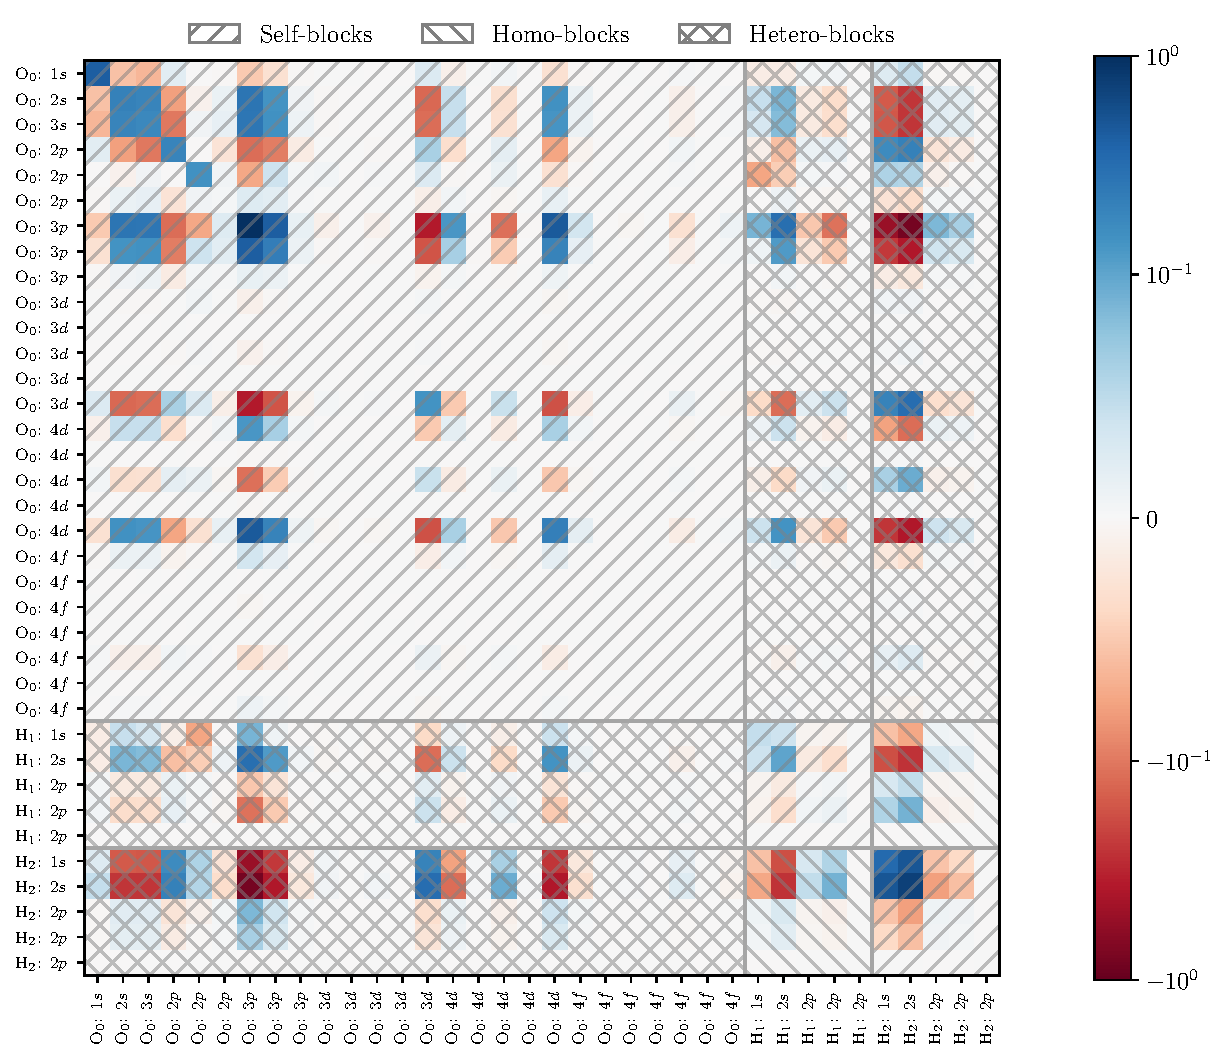
\includegraphics[width=\textwidth]{../fig/gnn/schematic_blocks.pdf}
    \caption[Matrix block regions of \ch{H2O}]{Converged density of \ch{H2O} with matrix block types indicated.}
    \label{fig:schematic_gnn_blocks}
\end{figure}
Evidently, the different block types vary widely in size. This needs to be addressed before feeding the data into the network. There are multiple ways of addressing this problem. A straightforward solution includes a simple zero pad to the maximum block size and subsequent masking. Another approach is the compression or transformation to a fixed size latent space or some sort of pooling to reach the desired input dimension. In order to not loose relevant data we take yet another route and encode each block using separate encoders. Via this approach we mitigate the problem of different sized inputs as long as the basis set is fixed. For the example in \autoref{fig:schematic_gnn_blocks} we would thus have four differently sized encoders (two for the self-blocks and one for homo-/ and hetero-blocks respectively). These encoders will transfer the input features into a common hidden dimension to be used in the network. After the propagation through our GNN the decoder side will decode the output dimension of our network to the respective block dimensions from which the whole matrix can be reconstructed.
\section{Preprocessing}
\label{sec:gnn_preproc}
Before feeding our data into the network we must bring it into a suitable form for learning with the \textsc{pytorch-geometric} framework \parencite{ref:PyTorchGeometric, ref:PyTorch_geom_paper}. After introducing the design of our data objects and graph creation we discuss a way to tackle the problem's sensitivity to spatial rotation before closing out with normalization and dataset creation remarks. 
\subsection{Graph creation}
\label{subsec:gnn_graph_creation}
A graph representation of our data is required which will be populated using the paradigms described in \autoref{sec:gnn_input_output_matrices}. Nodes of our graph are essentially represented by embeddings of our overlap self-blocks. This leaves us with one node per atom in our molecule. To enable easier benchmarking and training processes the targets (Fock- or density matrix-self blocks) are also stored in our graph object. Nodes are connected by directed edges which are given by an embedding of the homo- / hetero-block regions under a given restriction. The restriction on edge formation may be given by a distance cutoff (e.g. \SI{3}{\angstrom}), but not necessarily limited to that method. In particular, for bonds involving high-angular-momentum orbitals, the highly directed radial extension of the electronic wavefunction should also lead to an edge between these respective nodes. Edge formation can thus be controlled by a threshold with regard to the maximum value or another metric e.g. a matrix norm for a given interaction interaction block. A tensor of indices is used to represent the directed edges between nodes identified with said index. Every bond is represented by two directed edges to support bidirectional data exchange between nodes.\\

Additionally, to the node and edge embeddings of our inputs and targets we store node atom-symbols and edge-symbols (e.g. \ch{C}-\ch{O}) to match encoder / decoder later on in our network. Furthermore, we store global index information for both node and interaction blocks to facilitate matrix reconstruction from our block representation. 

\subsection{Data Augmentation}
\label{subsec:gnn_data_augmentation}
The input (overlap) as well as output (Fock / density matrix) are quantities which are not generally invariant under rotations of our molecular system. In essence this means that we must find a way to learn differently rotated molecules and produce their respective Fock / density matrices to later deduce our initial density. While the idea of making the input invariant under rotation, by using a predetermined standard orientation, was initially considered, problems arise with this approach. Most prominently, defining a standard orientation for isomers / isomer-parts, such as \ch{C7H10O2} or submolecules thereof, is far from trivial. Even if such a standard orientation is defined, one has to consider an additional pre- and post-processing step to rotate the input into the standard orientation and the output back to the original orientation. \\
Contrary to this, the model can learn differently rotated inputs to generate the corresponding outputs. This is achieved by augmenting the dataset with different rotations of the same molecules / submolecules. Rotating the input coordinates using a rotation matrix $R$ is in principle rather straightforward. However, the corresponding overlap, density and Fock matrices also have to be transformed accordingly or recalculated. The later is computationally not feasible, hence we use the corresponding Wigner D-matrices to transform input and output matrices. 
The Wigner D-matrix is a unitary matrix with $2L + 1$ rows and columns, where $L$ is the angular momentum. For a given rotation $R$ the Matrix elements of overlap, density and Fock matrix transform according to:
\begin{equation}
    \label{eq:wigner_d_transform}
    O'_{ij} = \sum_{k,l} \mathcal{D}^{(L)}_{ik}(R) O_{kl} \mathcal{D}^{(L)*}_{lj}(R)
\end{equation}
Naturally, the transformation only acts on spatial orbitals with no rotational symmetry along the axis of rotation (i.e. $L \neq 0$). Given the blocks defined in \autoref{sec:gnn_input_output_matrices} $\mathcal{D}^{(L)}$ will only transform elements of the blocks with at least one orbital having $L \neq 0$. \\


Concretely, the input data is augmented by sampling a random rotation axis, using 3 normally distributed values to obtain an axis and a random rotation angle $\theta \in [0, 2\pi]$. Given this axis and angle, the corresponding transformations are performed to the overlap, density and Fock matrices to obtain augmented samples. New graphs are created using these transformed matrices as explained in the precious section and added to the dataset. \\
Due to grid spacing in DFT calculations small deviations ($\approx 0,1 \unit{\milli\hartree}$ in the Fock matrix) between the transformed matrices and newly calculated ones using the rotated atom coordinates occur. These deviations only slightly affect the accuracy of the reconstructed density (see \autoref{eq:density_reconstruction_from_fock}) and are not relevant during training, as we evaluate the model against the provided target. In other words, if the model predicts the density via the Fock matrix, we compare it to a reference density that was also reconstructed from the (transformed) Fock, not from a directly transformed density matrix.\\
%! Note that translating the molecule should change absolutely nothing about the Overlap or Fock matrix. 

\subsection{Normalization \& data split}
\label{subsec:gnn_normalization}
Means and standard deviations are calculated on a per block-type basis (e.g. for the \ch{O}-\ch{H} hetero-block) on all training data samples. This is done for the input (overlap matrix) and the output / targets (Fock or density matrix).\\
It should be noted that the inclusion of data augmentation samples does not change these values besides machine precision errors. The normalization is then performed by subtracting the mean and dividing by the standard deviation for each block-type. To avoid numerical instabilities, especially for very sparse blocks (std. dev $\rightarrow 0$), a value of $10^{-6}$ is used should the standard deviation fall bellow this value for a given block. \\

The dataset is ultimately split into training, validation, and test sets, typically following a ratio of 80\% / 10\% / 10\%, where 100\% refers to the number of original (non-augmented) samples.

When applying a data augmentation factor of $1.5$, meaning that 50\% more samples are generated synthetically, the training set is extended to contain 120\% of the original data, while the validation and test sets remain unchanged at 10\% each. This ensures that evaluation is performed exclusively on the original, unaltered data and avoids any data leakage through augmented samples. To ensure comparability of benchmarks in \autoref{chap:application} the \textsc{scf\_guess\_datasets} package was used to obtain samples \parencite{ref:milacher_scf_guess_datasets}.

\section{ML pipeline \& GNN Design}
\label{sec:gnn_design}
The GNN's pipeline is designed to take coordinates from xyz-files, embed them into a graph form to facilitate training, and eventually obtain the full density matrix. A schematic overview of the pipeline is given in \autoref{fig:gnn_pipeline_design}

\begin{figure}[H]
    \centering
    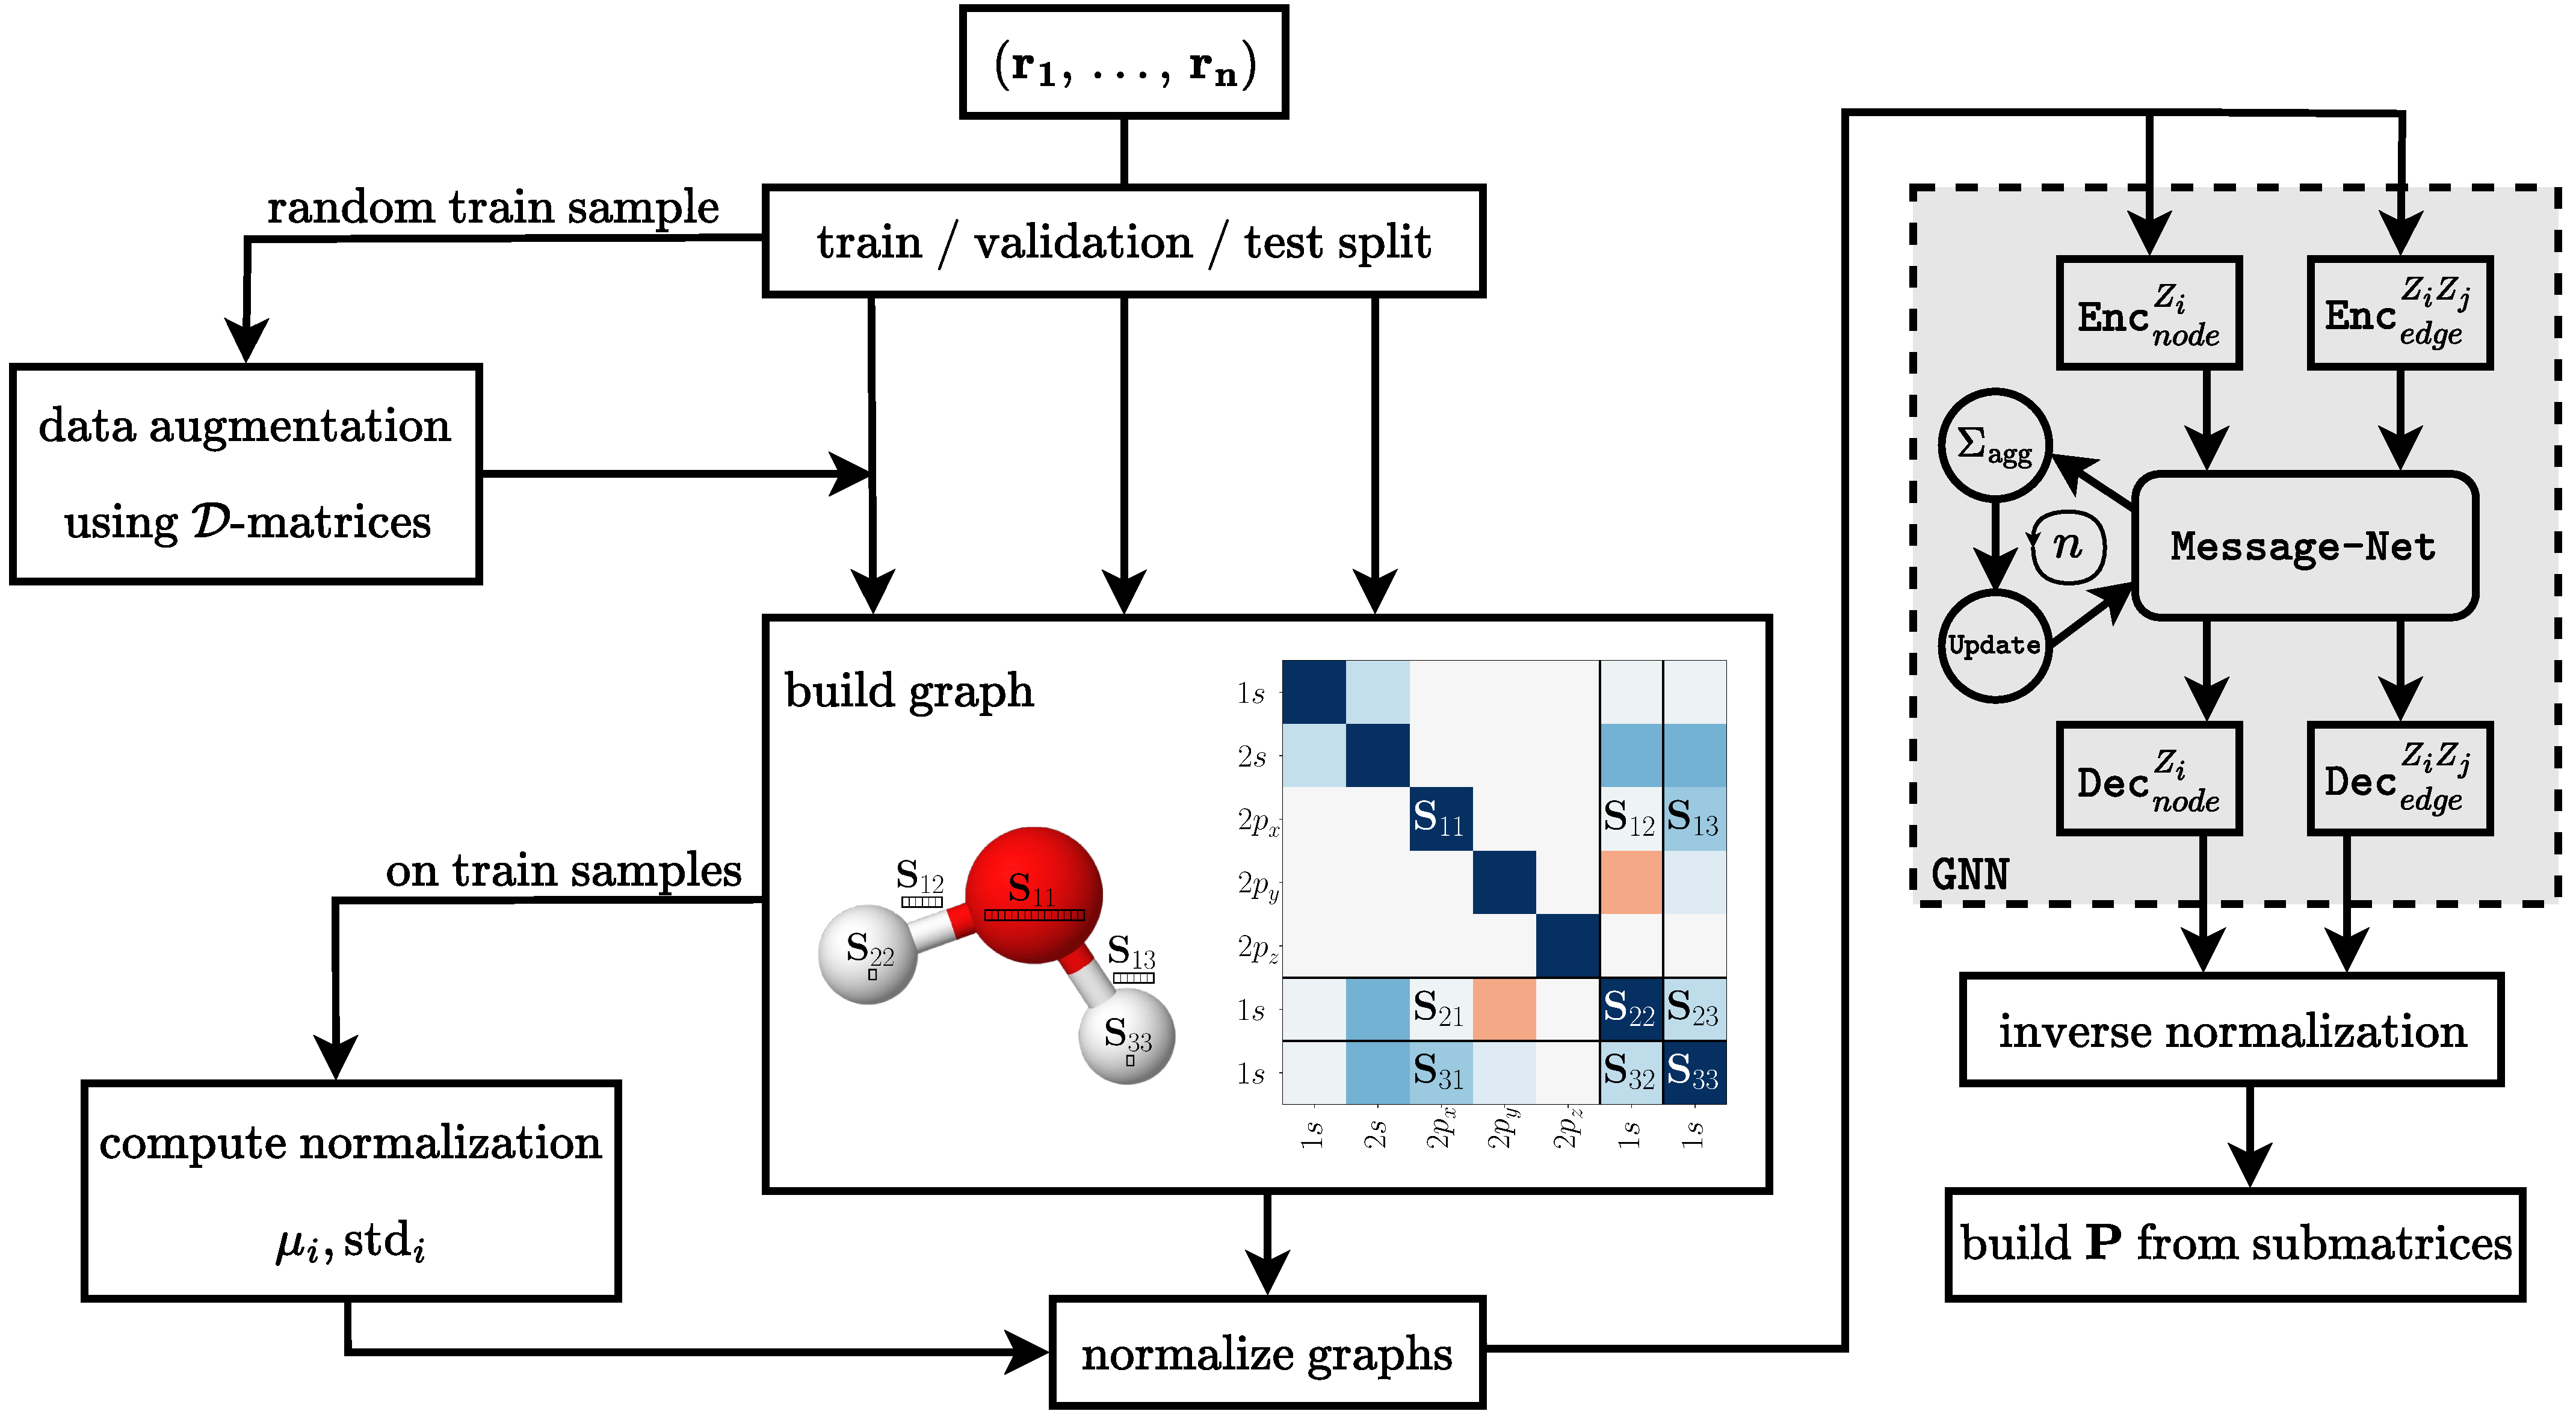
\includegraphics[width=\textwidth]{../fig/gnn/GNN_design.pdf}
    \caption[GNN pipeline design]{Overview of the GNN pipeline: training data is augmented, converted to graphs, normalized, and passed through a message-passing GNN. Predicted submatrices are denormalized and combined to reconstruct the full density matrix. \ch{H2O} overlap matrix is shown with exemplary embedding vectors for the STO-3G basis set.}
    \label{fig:gnn_pipeline_design}
\end{figure}

\textbf{Encoders}\\
To obtain a common input dimension differently sized blocks are encoded separately. Programmatically, this is enabled by a factory class that creates the required encoders for the different block types and sizes at runtime Given the \ch{H2O} example in \autoref{fig:schematic_gnn_blocks}, we obtain two encoders for the self-blocks, one for \ch{O}: $\texttt{Enc}^{8}_{node}$ and one for \ch{H}: $\texttt{Enc}^{1}_{node}$. The example above uses a cutoff distance of $\SI{1}{\angstrom}$ for the edge formation, which yields one edge encoder type for the \ch{O}-\ch{H} bonds: $\texttt{Enc}^{8\,1}_{edge}$. Due to the arguably small cutoff distance--in practice this will be set to higher values to capture interactions between orbitals of higher angular momentum with longer radial extension--there is no \ch{H}-\ch{H} edge encoder. \\
Node and edge encoders alike are implemented as a 2-layer network with a GeLU-activation between the layers. The first layer maps the input matrix to a fixed hidden dimension\footnote{For edge encoders, the interatomic distance is appended as an additional input feature.}, while the second layer maps from hidden dimension to hidden dimension. 

\textbf{Message Net (Message Passing)}\\
The Message Net is a simple feed forward network with a given linear layer depth GeLU activation and optional dropout, both fixed at initialization. It is designed to map an input of $3 \times$ the hidden dimension, which includes the node embeddings and the edge embedding of two connected nodes, to an output with size hidden dimension. This happens for each source-target node connection in the graph, in the example we `pass a message' from \ch{O} to \ch{H} and vice versa. Messages are only passed between nodes that are connected by an edge and never from one node to itself (i.e. there are no self-loops). All incoming messages are summed over per target node, for  example \ch{O} receives two messages from the \ch{H} atoms and each \ch{H} receive one from \ch{O}. A concatenation of the aggregated sum and the node embedding is fed into a node updater network which maps from twice the hidden dimension via a linear layer, GeLU activation and another linear layer back to one hidden dimension. When all node updates are completed, one round of message passing is finished. Multiple rounds of message passing are performed to enable information travel between more distant non-directly connected nodes.\\
Parameters mentioned above, such as the hidden dimension, number of message passing steps, dropout, etc. are all hyperparameters that can be tuned during training. 

\textbf{Decoder}\\
Decoders are effectively reversing the transformation of the encoders to obtain the original dimensions of the matrix blocks. This preferably results in accurate target predictions. Node decoders, like $\texttt{Dec}^{8}_{node}$ or  $\texttt{Dec}^{1}_{node}$, map back to the upper triangular matrix of self-blocks, while edge decoders, such as $\texttt{Dec}^{8\,1}_{edge}$, to the full interaction matrix. Both use one linear layer which directly maps from the hidden dimension to the respective output dimension. \\

The raw output of the GNN needs to be inversely normalized to yield meaningful predictions. Ultimately, the full matrix is rebuild from self-blocks and interaction blocks by reversing the block splitting procedure described in \autoref{sec:gnn_input_output_matrices}. If the target is the Fock matrix, the reconstruction of the density matrix is performed as a post-processing step.

\section{Training}
\label{sec:gnn_training}

The GNN is trained using various hyperparameters and configurations to optimize its performance on different datasets. While details on the application of the network will be given in \autoref{chap:application}, the general training procedure will be discussed in this section. \\

\textbf{Loss Function}\\
Practically the choice of the loss function can also be handled as a hyperparameter. While a physically motivated loss function which correlates well with the iteration count is preferable, it is far from trivial to derive such a metric. A variety of these metrics\footnote{For example F-score for different guessing schemes in \autoref{chap:fock_matrix_predictions}} were initially promising when scoring guesses against converged density, but turned out to be suboptimal in terms of correlation to iteration count. \\
If not mentioned otherwise in the later subchapters MSE (see \autoref{subsec:background_loss_function}) will be used as a loss function. While this function may not offer a direct physical interpretation, besides the total global `overlap' of prediction and target matrices, it is well understood and established in a wide variety of learning problems. Additionally, the loss function, which is evaluated block-wise\footnote{block-wise evaluation is computationally also easier because the full density matrix isn't reconstructed during training} on the target matrices, can be combined and/or weighted in various ways to obtain a single scalar loss value per sample. 

\textbf{Optimizer \& learn rate \& early stopping}\\
Similar to the loss function, the optimizer could also be treated as a hyperparameter. However, due to computational and time constraints, it will be fixed for the scope of this thesis. A stochastic gradient descent optimizer, namely AdamW, is used in all training runs in combination with a learn rate scheduler. AdamW is preferred over the initial Adam implementation due to the decoupling of weight decay in AdamW \parencite{ref:adamW}. All parameters in the learn rate scheduler (reduction factor, patience, threshold, etc.) and the initial learn rate are also treaded as hyperparameters. \\
Training trials during which the validation loss stagnates will be cut short using the grace-epochs parameter. In most systems with high atom-counts our model learns sufficiently fast. This is due to the fact that each sample contains multiple self- and interaction blocks per atom sort / atom combination. Therefore, the number of grace epochs are set to a rather low 5 epochs in most runs. 

\textbf{Hyperparameter tuning}\\
Hyperparameter tuning is performed using the Ray Tune \parencite{ref:ray_tune} package. Given the the huge variety of hyperparameters\footnote{even with the shared encoder / decoder architecture of the GNN} a grid search is computationally not feasible. The Asynchronous Successive Halving Algorithm (ASHA) is used as a scheduler to find suitable hyperparameter combinations faster. The authors claim that the algorithm finds good hyperparameters nearly an order of magnitude faster, compared to a random search. \parencite{ref:ASHA}\\
To further cut down on discrete combinations, ASHA samples hyperparameters by drawing values uniformly or log-uniformly from an interval or by randomly selecting from a predefined list; some hyperparameters remain fixed during this process. This constitutes a resource efficient way, which can be easily extended to larger search spaces and larger compute clusters if needed. 

\section{Benchmark model}
\label{sec:0_d_benchmark_model}
Since loss and iteration count aren't inherently correlated, we must validate our model by actually running SCF calculations using its predicted densities. This computationally rather expensive step can only be performed on selected model, meaning Hyperparameter tuning cannot directly benefit from actual iteration counts obtained by new calculations.\\
Comparable to the benchmarks in \autoref{chap:fock_matrix_predictions}, we will benchmark the GNN against established PySCF guesses. Additionally, we introduce an element-wise average guess called $\overline{P}$ in \autoref{eq:avg_guess}: 

\begin{equation}
    \label{eq:avg_guess}
    \overline{P}_{\mu\nu} = \frac{1}{N_\text{train}} \sum_{i=1}^{N_\text{train}} P^{(i)}_{\mu\nu}
\end{equation}
For fairness this average is only evaluated on the elements of the respective training set. The performance of $\overline{P}$ guess and various PySCF schemes on the \ch{C7H10O2} isomer test subset is given in \autoref{fig:dummy_iterations_qm9_isomers}. 
\begin{figure}[H]
    \centering
    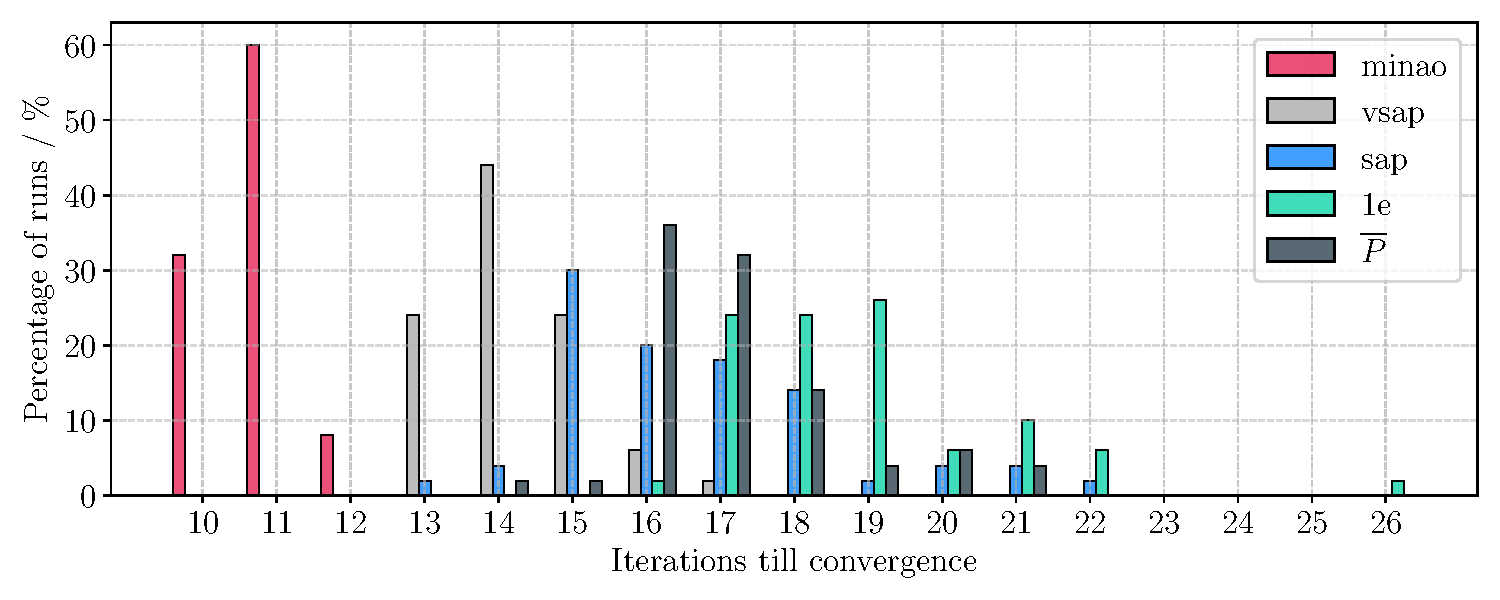
\includegraphics[width=\textwidth]{../fig/gnn/0_d_model_iteration_count_bar.pdf}
    \caption[Iterations till convergence distribution for QM9-isomers]{Iterations till convergence distribution for QM9-isomers for PySCF and $\overline{P}$ guesses.}
    \label{fig:dummy_iterations_qm9_isomers}
\end{figure}

For further insights regarding convergence behavior using a second order newton solver, refer to \autoref{sec:notes_on_so_newton} 